\section{Task Consola}

En este ejercicio programamos la tarea \texttt{Task Consola}, que lo que hace es simular una tarea interactiva que realiza $n$ llamadas bloqueantes con una duración de ticks de reloj aleatoria entre \texttt{bmin} y \texttt{bmax}.

Una llamada se clasifica como \texttt{bloqueante} cuando el procesador no puede seguir ejecutando instrucciones hasta que algun tipo de recurso este disponible. Las llamadas bloqueantes en general son de entrada y salida. Este tipo de recursos se acceden comunmanete mediante un \texttt{syscall}. El \texttt{syscall} en si debe ser ejecutado en primera instancia, lo que asumiremos que toma un ciclo de reloj. Luego el recurso toma un total de $t$ ticks de reloj de forma aleatoria en responder. Por lo tanto, una tarea ineractiva toma un ciclo de reloj para la llamada y permanecera bloqueada durante $t$ ciclos adicionales.

\subsection{Código}

\begin{lstlisting}[language=C++, breaklines=true]
void TaskConsola(int pid, vector<int> params) {
	srand(1); // set seed

	for (int i = 0; i < params[0]; ++i) {
		int t = params[1] + rand() % (params[2] - params[1] + 1);
		uso_IO(pid, t);
	}
}
\end{lstlisting}

Esta tarea toma un \texttt{pid} y un vector \texttt{params} de 3 parámetros. Dado que nuestros resultados dependerán de un generador de números pseudo-aleatorio, setteamos una semilla con el objetivo de poder replicar nuestros resultados.

Luego, el loop ejecuta la llamada \texttt{bloqueante} simulada con un request de entrada/salida utilizando como parámetro un numero aleatorio entre \texttt{bmin} y \texttt{bmax} que se encuentran en el vector en ese orden respectivamente.

Este numero no necesariamente tiene una distribución uniforme perfecta, pero se le parece demasiado dado que genera un valor entre $0$ y \texttt{RAND\_MAX}\footnote{http://www.cplusplus.com/reference/cstdlib/RAND\_MAX} (definido en la std) y luego le aplica la función modulo con un numero chico a un dominio grande. La función devuelve un numero $t \in [0, RAND\_MAX]$. La función modulo luego achica ese dominio a $[0, bmax - bmin]$. Finalmente, al sumarle bmin logramos que $t \in [bmin, bmax]$.

\subsubsection{Diagrama GANTT}

El siguiente diagrama fue generado con los siguientes parametros:

\begin{enumerate}
	\item lote\_tsk: 1.tsk
	\item num\_cores: 1
	\item switch\_cost: 0
	\item sched\_class: SchedFCFS
	\item n: 10
	\item bmin: 1
	\item bmax: 10
\end{enumerate}

\begin{figure}[h]
    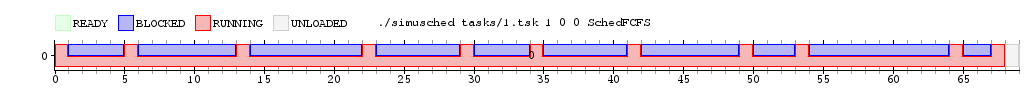
\includegraphics[width=\linewidth]{images/1.png}
    \label{fig:Task Consola}
    \caption{Task Consola}
\end{figure}

\textbf{TODO: Explicar bien el diagrama!}